\section{Stochastic Slow}
\label{sec:1STS}

Stochastic Slow jest wolniejszą wersja podstawowego oscylatora stochastycznego. Składa się z dwóch linii oscylacyjnych: głównej linii oscylatora tzw. \%K oraz pomocniczej wygładzonej postaci tej linii tzw. \%D. Obie linie osiągają wartości z przedziału 0 - 100.  Sposób wyliczenia kolejnych wartości obu linii dla danego punktu w czasie przedstawiają wzory \ref{wzor_1} oraz \ref{wzor_2}.
\begin{equation}
\%K = \left[\begin{array}{c} \frac{ \sum_{j=0}^{2} (C_j - min(L_j, n))}{ \sum_{j=0}^{2} (max(H_j, n) - min(L_j, n))}\end{array}\right]\\
\label{wzor_1}
\end{equation}
\begin{equation}
\%D = SMA(\%K, 3)
\label{wzor_2}
\end{equation}

\noindent Dodatkowo mogą być poszukiwane dywergencje względem wykresu cenowego. Możliwe jest też poszukiwanie tzw. odwróconych dywergencji. W tej wersji wskaźnik może być używany jako miernik wykupienia / wyprzedania rynku. Wadą wskaźnika jest to, że w mocnych ruchach trendowych skrajne stany rynku mogą być sygnalizowane przedwcześnie.
Przy interpretacji wskaźnika najważniejszy jednak jest fakt, że wskazuje on momenty w których mogą być zawierane transakcje. Podstawowa zasada zakłada przyjęcie jako sygnału kupna sytuację gdy występują przecięcia linii \%D przez linię \%K od dołu. Natomiast, gdy linia \%D jest przecinana przez linię \%K od góry, to przyjmuje się taką sytuację za sygnał sprzedaży. Zostało to przedstawione na rysunku \ref{zasada}. \\
\begin{figure}[h!]
\centering
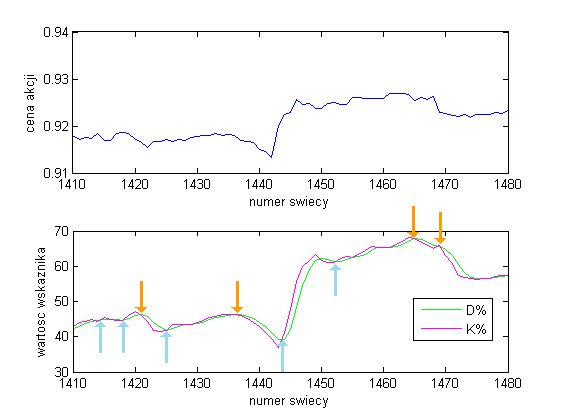
\includegraphics[width = \textwidth]{ss.png}
\caption{Fragment przebiegu kursu akcji (górny wykres) oraz odpowiadające jemu linie \%K i \%D wraz z sygnałami kupna --- błękitne strzałki oraz sygnałami sprzedaży --- pomarańczowe strzałki (dolny wykres)}
\label{zasada}
\end{figure}
\FloatBarrier

\noindent Poniższy listing przedstawia zaimplementowaną w środowisku MATLAB strategię wykorzystującą opisywany wskaźnik.
\begin{scriptsize}
\begin{lstlisting}
maxes=zeros(candlesCount,1);
mins=zeros(candlesCount,1);
K=zeros(candlesCount,1);
D=zeros(candlesCount,1);
kon=candlesCount-1;
for i=4:kon
    maxes(i) = max(verificationC(i-min(i-1,paramMALength):i-1,2));
    mins(i) = min(verificationC(i-min(i-1,paramMALength):i-1,3));
    K(i) = 100 * (sum(verificationC(i-min(i-1,3):i-1,4)-mins(i-min(i-1,2):i)) / sum(maxes(i-min(i-1,2):i)-mins(i-min(i-1,2):i)));
    D(i) = sum(K(i-min(i-1,2):i)) / min(i-1,3);
end

sumR=zeros(1,candlesCount);
R=zeros(1,candlesCount);
pocz=max(paramMALength, 10)+3;
iL=0; %liczba otwieranych pozycji kupna
iS=0; %liczba otwieranych pozycji sprzedarzy
lastCandle = kon-paramMALength;
recordReturn=0;  %rekord zysku
recordDrawdown=0;  %rekord obsuniecia
LastPos = 0; % zmienna do prz echowywa nia warto ś ci na otwarciu ostatniej pozycji
for i=pocz:lastCandle
    
    if K(i-1) < D(i-1) && K(i) >= D(i) % warunek kupna
        R(i)= - C(i+1,4)+LastPos-spread; % zamknięcie S
        LastPos = C(i+1,1); % otwarcie L
        iL=iL+1;
    elseif K(i-1) > D(i-1) && K(i) <= D(i) % warunek sprzedaż y
        R(i)=C(i+1,4)-LastPos-spread; % zamknięcie L
        LastPos = C(i+1,1); % otwarcie S
        iS=iS+1;
    end
    sumR(i)= sum(R(pocz:i));  %krzywa narastania kapitału
    
    if sumR(i)>recordReturn
        recordReturn=sumR(i);
    end
    
    if sumR(i)-recordReturn<recordDrawdown
        recordDrawdown=sumR(i)-recordReturn;  %obsuniecie maksymalne
    end
end

%wyniki końcowe
sumReturn=sumR(lastCandle);
Calmar=-sumReturn/recordDrawdown;  %wskaznik Calmara
\end{lstlisting}
\end{scriptsize}


Na podstawie zebranych informacji dotyczących wskaźnika $Stochastic Slow$ utworzono prostą strategię inwestycyjną bazującą na regule: jeśli linia $\%D$ jest przecinana przez  linię $\%K$ od dołu, to otwierana jest pozycja długa ($L$), a zamykana pozycja krótka ($S$), która została wcześniej otwarta. Natomiast gdy linia \%D jest przecinana przez linię \%K od góry, to otwarta zostanie pozycja krótka, a zamknięta długa. Badania zostały przeprowadzone na parze walutowej $CADCHF$ (szereg czasowy przedstawiony na rysunku \ref{rys2}). \\
\begin{figure}[h!]
\centering
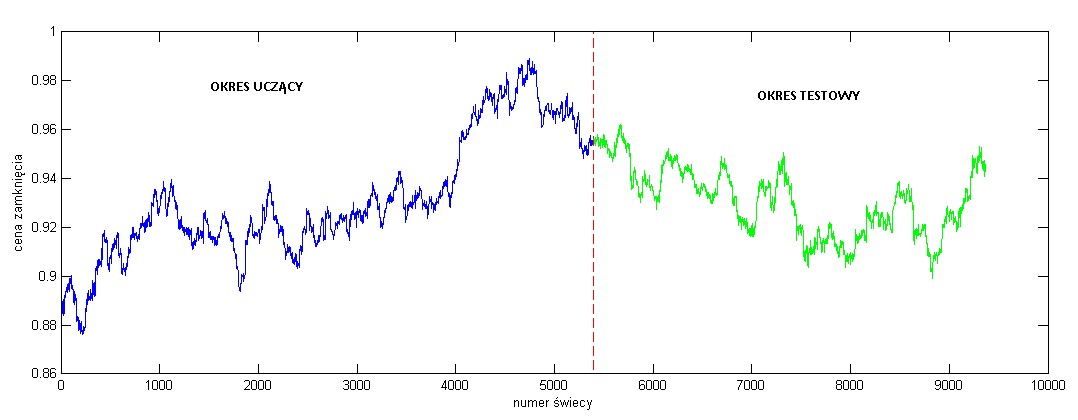
\includegraphics[width = \textwidth]{szereg.png}
\caption{Badany szereg czasowy z podziałem na część uczącą i testową}
\label{rys2}
\end{figure}
\FloatBarrier
Cały zbiór danych (świec) podzielony został na dwie części: uczącą ($60\%$ całości) oraz testową ($40\%$ całości). W przeprowadzonych badaniach poszukiwano optymalnej wartości parametru $n$ na okresie uczącym, następnie weryfikowano otrzymane wyniki na okresie testowym. Wybór optymalnej wartości parametru $n$ determinowano na dwa sposoby:
\begin{itemize}
\item otrzymanego zysku skumulowanego,
\item wskaźnika Calamara.
\end{itemize}

\noindent \textbf{I Wyniki badań przy maksymalizacji po zysku.}\\
\begin{figure}[h!]
\centering
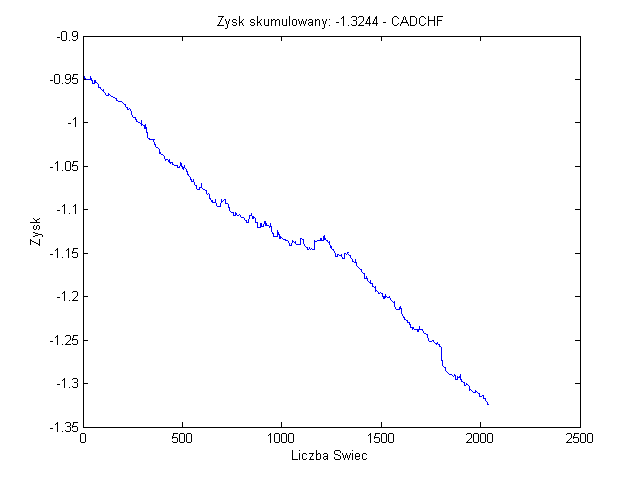
\includegraphics[width = 0.6\textwidth]{SS_CADCHF_S4LS_zysk.png}
\caption{Zysk skumulowany CADCHF na okresie testowym przy maksymalizacji według zysku}
\end{figure}
\FloatBarrier
\begin{verbatim}
OKRES UCZĄCY
Zysk skumulowany:     0.2917
Calmar:     0.4538
Liczba otwartych pozycji długich:     400
Liczba otwartych pozycji krótkich:     405

OKRES WALIDUJĄCY
Zysk skumulowany:     -1.3244
Calmar:     -1
Liczba otwartych pozycji długich:     244
Liczba otwartych pozycji krótkich:     245
\end{verbatim}
\newpage
\textbf{II Wyniki badań przy maksymalizacji po wskaźniku Calmara.}\\
\begin{figure}[h!]
\centering
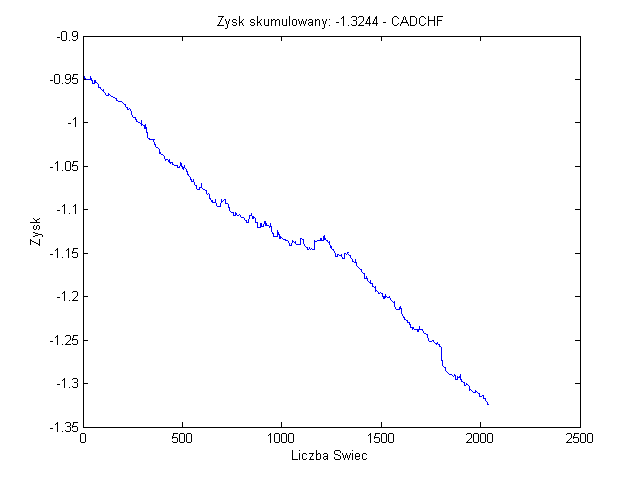
\includegraphics[width = 0.6\textwidth]{SS_CADCHF_S4LS_calmar.png}
\caption{Zysk skumulowany EURJPY na okresie testowym przy maksymalizacji według Calmara}
\end{figure}
\FloatBarrier
\begin{verbatim}
OKRES UCZĄCY
Zysk skumulowany:     0.2917
Calmar:     0.4538
Liczba otwartych pozycji długich:     400
Liczba otwartych pozycji krótkich:     405

OKRES WALIDUJĄCY
Zysk skumulowany:     -1.3244
Calmar:     -1
Liczba otwartych pozycji długich:     244
Liczba otwartych pozycji krótkich:     245
\end{verbatim}
%
